\documentclass{beamer}
\usepackage{ctex}

\usetheme{metropolis}
\usepackage{appendixnumberbeamer}

\usepackage{booktabs}
\usepackage[scale=2]{ccicons}

\usepackage{pgfplots}
\usepgfplotslibrary{dateplot}

\usepackage{xspace}
\usepackage{graphicx}

\usepackage[style=verbose,backend=bibtex]{biblatex}
\addbibresource{../paper/Biblio/ref.bib}

\newcommand{\themename}{\textbf{\textsc{metropolis}}\xspace}

\def\signed #1{{\leavevmode\unskip\nobreak\hfil\penalty50\hskip2em
\hbox{}\nobreak\hfil(#1)%
\parfillskip=0pt \finalhyphendemerits=0 \endgraf}}

\newsavebox\mybox
\newenvironment{aquote}[1]
{\savebox\mybox{#1}\begin{quote}}
{\signed{\usebox\mybox}\end{quote}}

\title{Metropolis}
\title{裸金属二进制翻译器的设计和实现}
\date{\today}
\author{Martins3}
\institute{The Open Source Community}
% \titlegraphic{\hfill\includegraphics[height=1.5cm]{logo.pdf}}

\begin{document}

\maketitle

\begin{frame}{目录}
	\setbeamertemplate{section in toc}[sections numbered]
	\tableofcontents[hideallsubsections]
\end{frame}

\section{研究背景}
\begin{frame}{二进制翻译器的应用场景}
	\begin{itemize}
		\item 安全,逆向,性能和调试
		\item \textbf{跨架构}
	\end{itemize}
\end{frame}

\begin{frame}{跨架构二进制翻译器}
	任何指令集架构初期都需要一个二进制翻译器
	\begin{itemize}
		\item 没有硬件的情况下,软件工程师可以在二进制翻译器上开发操作系统。
		\item 软件适配需要时间。 Apple 使用 Rosetta 2 让软件厂商有时间适配 ARM 架构的 Mac 。
	\end{itemize}

	龙芯推出了基于 LoongArch 架构的 3A5000,相较于上一代的基于 MIPS 架构的 3A4000,有 50\% 的性能提升。
\end{frame}

\begin{frame}{跨架构二进制翻译}
	\begin{figure}
		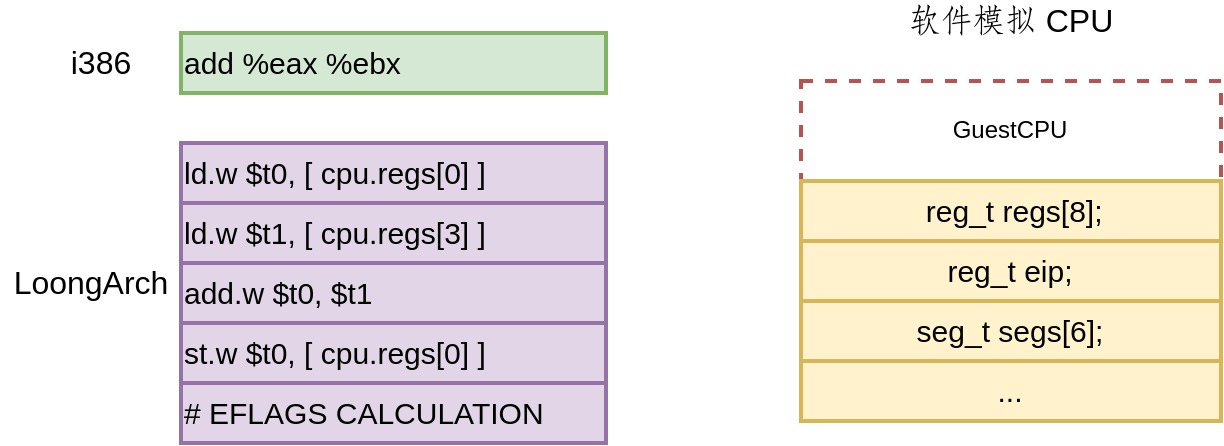
\includegraphics[width=0.8\linewidth]{../paper/images/basic-flow.jpg}
		\caption{将一条 x86 指令翻译成为 LoongArch 指令}
	\end{figure}
	\begin{itemize}
		\item 使用软件模拟硬件。
		\item 根据指令手册使用宿主机(Host)指令模拟客户机(Guest)指令。
	\end{itemize}
\end{frame}

\begin{frame}{静态二进制翻译}
	\begin{figure}
		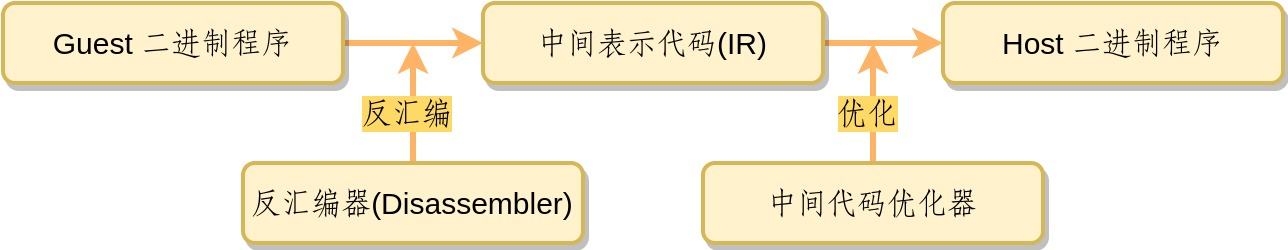
\includegraphics[width=1\linewidth]{../paper/images/static-bt.jpg}
		\caption{静态二进制翻译器执行流程}
	\end{figure}
	静态二进制翻译在 Guest 程序执行之前完成所有的翻译工作,因为缺乏运行时信息,能够翻译的 Guest 程序类型有限。
\end{frame}

\begin{frame}{动态二进制翻译}
	\begin{figure}
		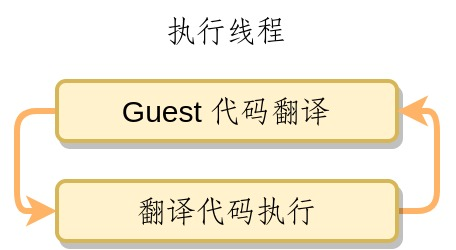
\includegraphics[width=0.4\linewidth]{../paper/images/basic-flow2.jpg}
		\caption{动态二进制翻译器执行流程}
	\end{figure}
	动态二进制翻译器采取边翻译边执行的模式,利用运行时信息来指导下一步的翻译。
\end{frame}

\begin{frame}{动态跨架构二进制翻译的优化: 翻译代码缓存}
	\begin{figure}
		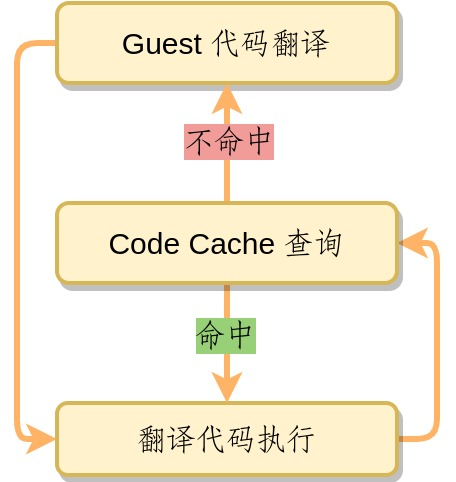
\includegraphics[width=0.3\linewidth]{../paper/images/basic-flow3.jpg}
		\caption{含有 Code Cache 的执行流程}
	\end{figure}
	翻译过的 Guest 代码无需重复翻译,当下次执行的时候可以直接使用缓存的翻译代码(Code Cache)。
\end{frame}

\begin{frame}{动态跨架构二进制翻译的优化: 翻译代码链接}
	\begin{figure}
		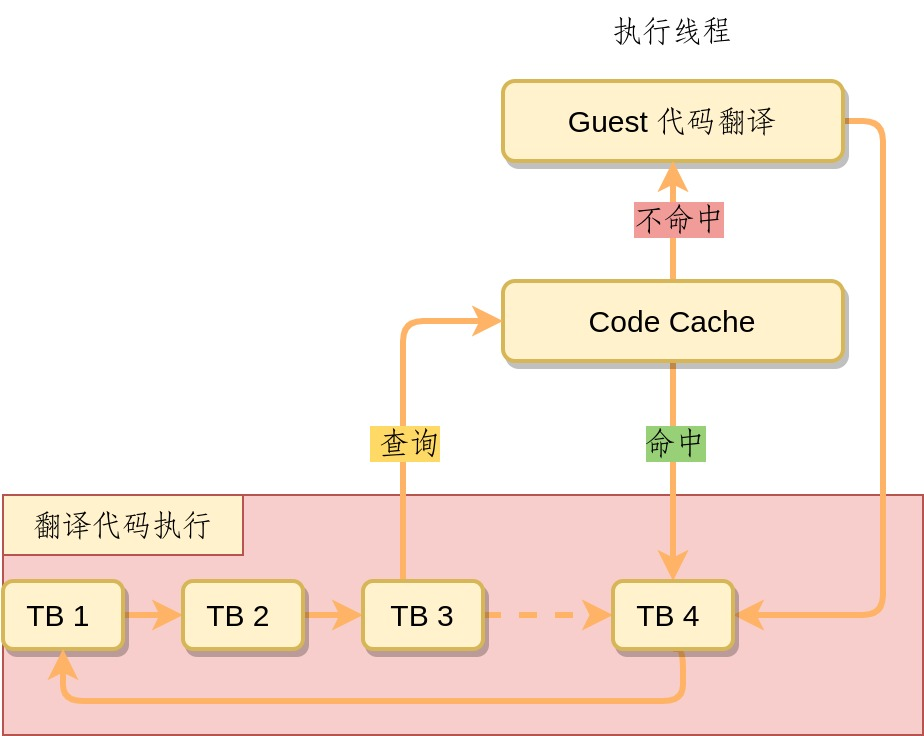
\includegraphics[width=0.5\linewidth]{../paper/images/basic-flow4.jpg}
		\caption{含有 TB Chain 的执行流程}
	\end{figure}
	最长的连续的不含有分支的指令构成一个翻译基本块 (Translation Block, 简称 TB)。
	将 TB 链接起来从而消除 Guest 和 Host 的上下文切换。
\end{frame}

\begin{frame}{系统级和进程级二进制翻译对比}
	\begin{figure}
		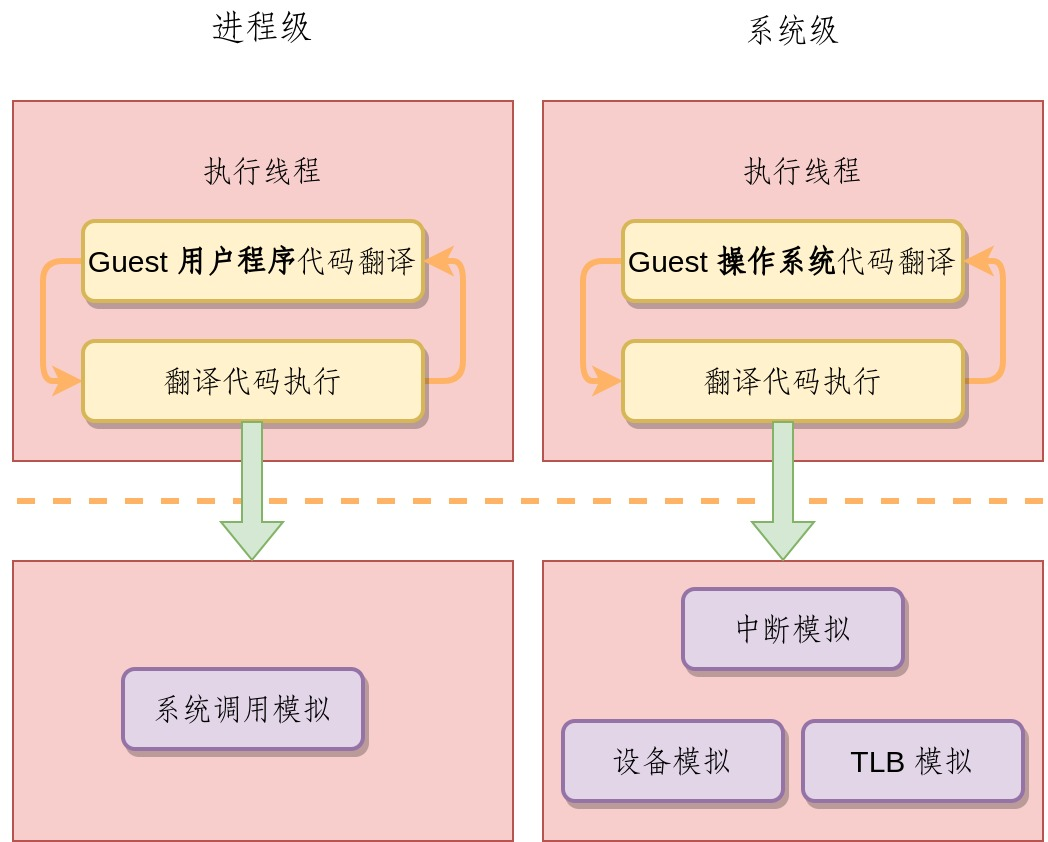
\includegraphics[width=0.5\linewidth]{../paper/images/user-sys-flow.jpg}
		\caption{系统级和进程级二进制翻译的执行流程}
	\end{figure}
	基本流程相同,但是系统级二进制翻译器无需模拟系统调用,但是需要模拟设备,TLB 和中断。
\end{frame}

\begin{frame}{进程级二进制翻译器的问题}
	\begin{columns}[T,onlytextwidth]
		\column{1.0\textwidth}
		\begin{alertblock}{}
			\begin{itemize}
				\item 如果想要 x86 Window 程序运行在 LoongArch Linux 上需要引入 Wine 来模拟操作系统的差异。
				\item 4K页 Guest 运行在 16K 页的 Host 上,需要特殊的处理。
			\end{itemize}
		\end{alertblock}
	\end{columns}
\end{frame}

\begin{frame}{系统态二进制翻译的挑战}
	\begin{columns}[T,onlytextwidth]
		\metroset{block=fill}
		\column{1.0\textwidth}
		\begin{block}{CPU}
			指令增多,部分指令在系统态有额外的语义
		\end{block}

		\begin{alertblock}{设备}
			\begin{itemize}
				\item 模拟设备,然后将设备的请求转发给 Host 操作系统
			\end{itemize}
		\end{alertblock}

		\begin{alertblock}{中断}
			\begin{itemize}
				\item Host 接收中断,模拟中断控制器,然后注入到 Guest 中
			\end{itemize}
		\end{alertblock}

		\begin{alertblock}{访存}
			\begin{itemize}
				\item 使用软件 TLB 实现虚实地址转换
			\end{itemize}
		\end{alertblock}
	\end{columns}
	这些挑战导致系统级二进制翻译器的性能低于进程级二进制翻译器,裸金属二进制翻译器(简称 BMBT)尝试解决这些挑战。
\end{frame}

\section{相关工作}

\begin{frame}{Transmeta Code Morphing}
	\begin{figure}
		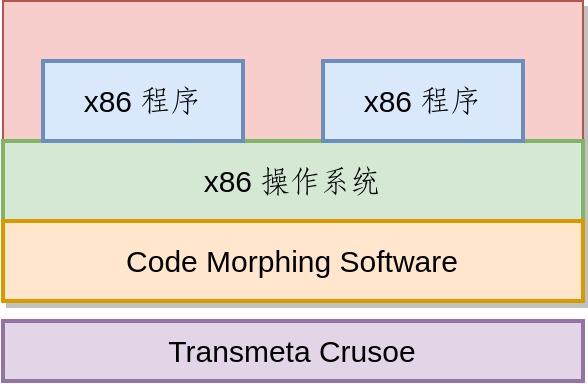
\includegraphics[width=0.4\linewidth]{../paper/images/transmeta.jpg}
		\caption{Transmeta Cursoe \& CMS }
	\end{figure}
	\begin{enumerate}
		\item x86 指令翻译为 VLIW 架构指令。
		\item 额外的硬件支持加速二进制翻译。
	\end{enumerate}
\end{frame}

\begin{frame}{QEMU}
	\begin{figure}
		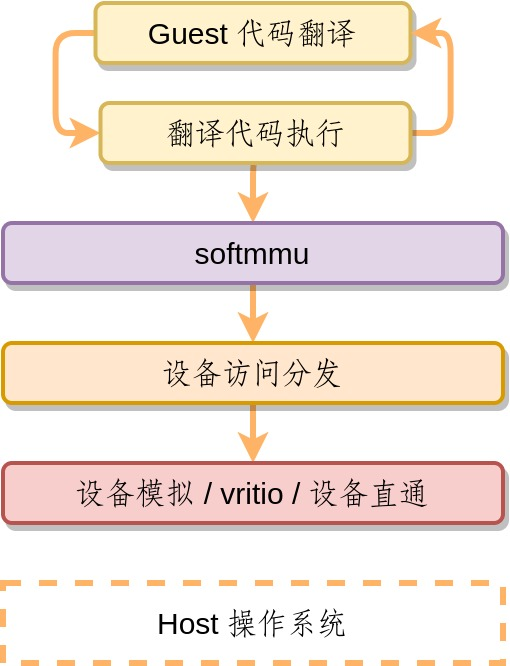
\includegraphics[width=0.3\linewidth]{../paper/images/device-virtualization.jpg}
		\caption{QEMU 软件架构}
	\end{figure}
	\begin{enumerate}
		\item 支持 20 种架构之间的互相翻译。
		\item 运行在用户态,利用操作系统来访问硬件来模拟 Guest 需要的资源。
	\end{enumerate}
\end{frame}

\begin{frame}{Captive}
	\begin{figure}
		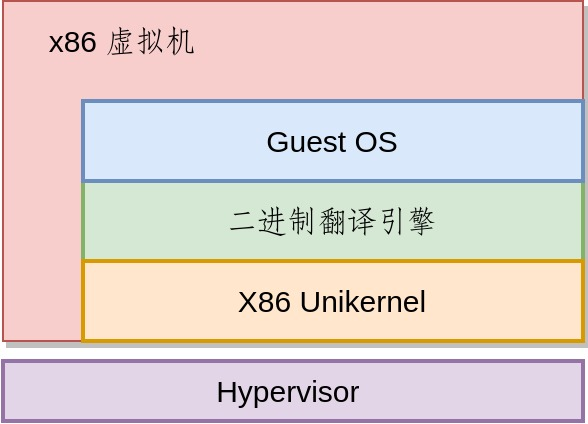
\includegraphics[width=0.5\linewidth]{../paper/images/captive.jpg}
		\caption{Captive 软件架构}
	\end{figure}
	\begin{enumerate}
		\item 将 arm 翻译为 x86 。
		\item 通过硬件辅助虚拟化的 Hypervisor 将二进制翻译器放到 non-root 态中的系统态中,从而直接访问硬件资源。
	\end{enumerate}
\end{frame}

\begin{frame}{现有方案的问题}
	\begin{itemize}
		\item Transmeta CMS 需要额外的硬件支持,此外 Cursoe 是 VLIW 架构,对于乱序多发射架构 CPU 下的二进制翻译器参考意义不大。
		\item QEMU 运行在用户态,难以消除操作系统的软件栈和用户态系统态上下文切换。
		\item Captive 等利用硬件辅助虚拟化直接访问硬件资源,但是虚拟机退出的开销不可忽视。
	\end{itemize}
\end{frame}

\section{裸金属二进制翻译器}
\begin{frame}{为何将二进制翻译器直接运行在系统态中}
	\begin{itemize}
		\item 只有一个地址空间,没有系统态和用户态之间的上下文切换,没有 TLB miss 。
		\item 消除操作系统的软件栈。
		\item 直接访问硬件,可以实现设备直通和硬件 TLB 访存加速。
	\end{itemize}
\end{frame}

\begin{frame}{BMBT 软件架构}
	\begin{figure}
		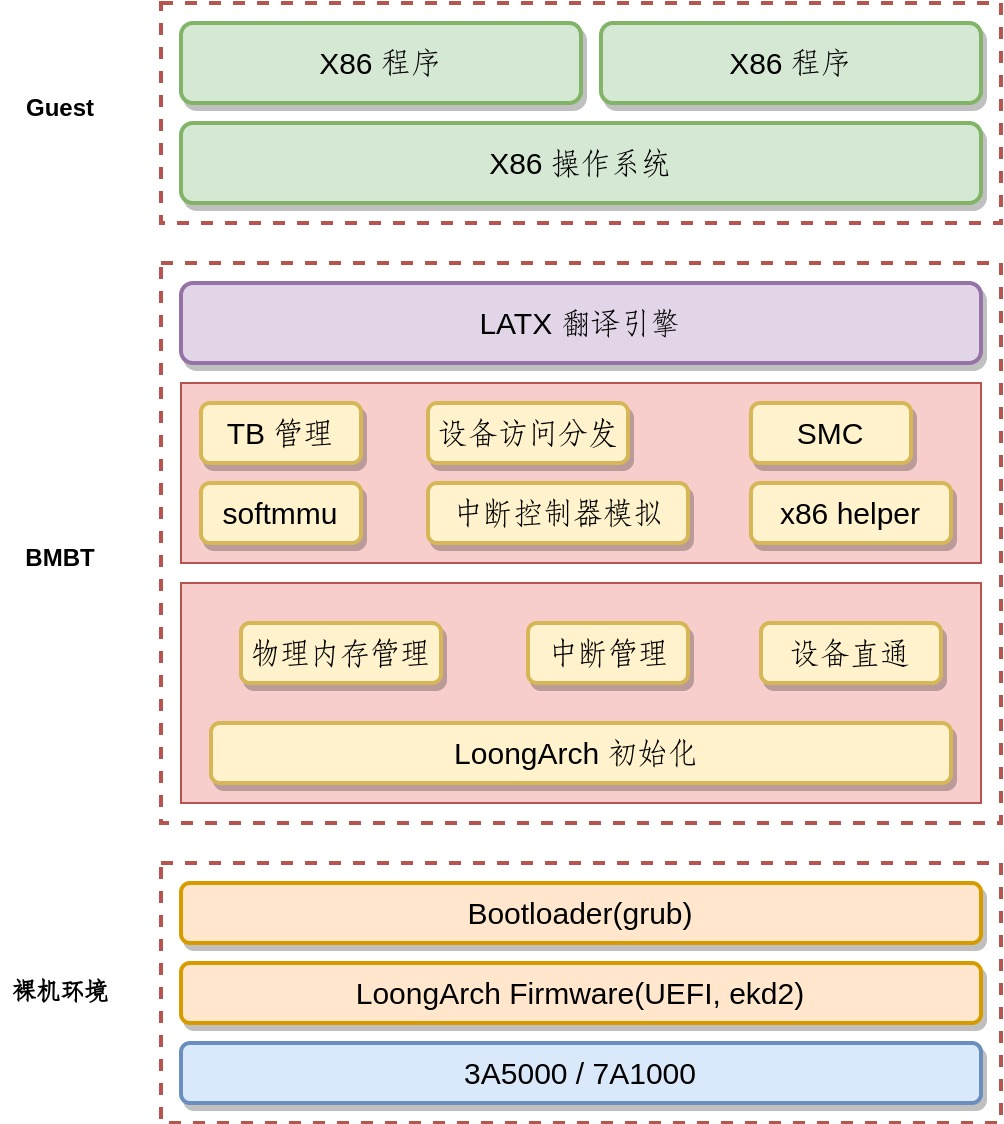
\includegraphics[width=0.6\linewidth]{../paper/images/bmbt.jpg}
	\end{figure}
\end{frame}


\begin{frame}{CPU 虚拟化}
	\begin{figure}
		
\includegraphics[width=\linewidth]{../paper/images/tcg.jpg}
		\caption{QEMU TCG}
	\end{figure}
	QEMU 为了实现多个架构之间的互相翻译,采用了 Tiny Code Generator(简称 TCG )作为中间指令。
\end{frame}

\begin{frame}{CPU 虚拟化}
	\begin{figure}
		
\includegraphics[width=\linewidth]{../paper/images/latx.jpg}
		\caption{LATX}
	\end{figure}
	LATX 是直接从 x86 到 LoongArch 的指令翻译引擎。
\end{frame}

\begin{frame}{设备虚拟化}
	\begin{figure}
		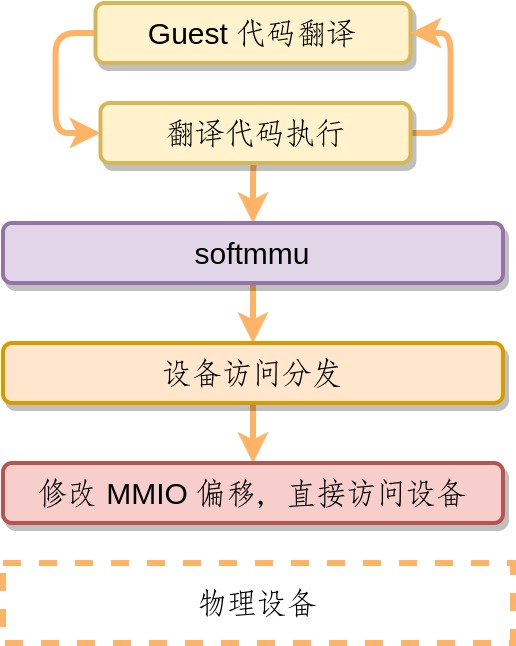
\includegraphics[width=0.3\linewidth]{../paper/images/bmbt-device.jpg}
		\caption{BMBT 设备虚拟化}
	\end{figure}
	包括 PCIe 在内的大多数设备都是架构无关的,BMBT 无需实现设备复用,因此可以让 Guest 直接操控设备,实现设备直通。
\end{frame}

\begin{frame}{设备虚拟化: PCIe 设备虚拟化}
	\begin{figure}
		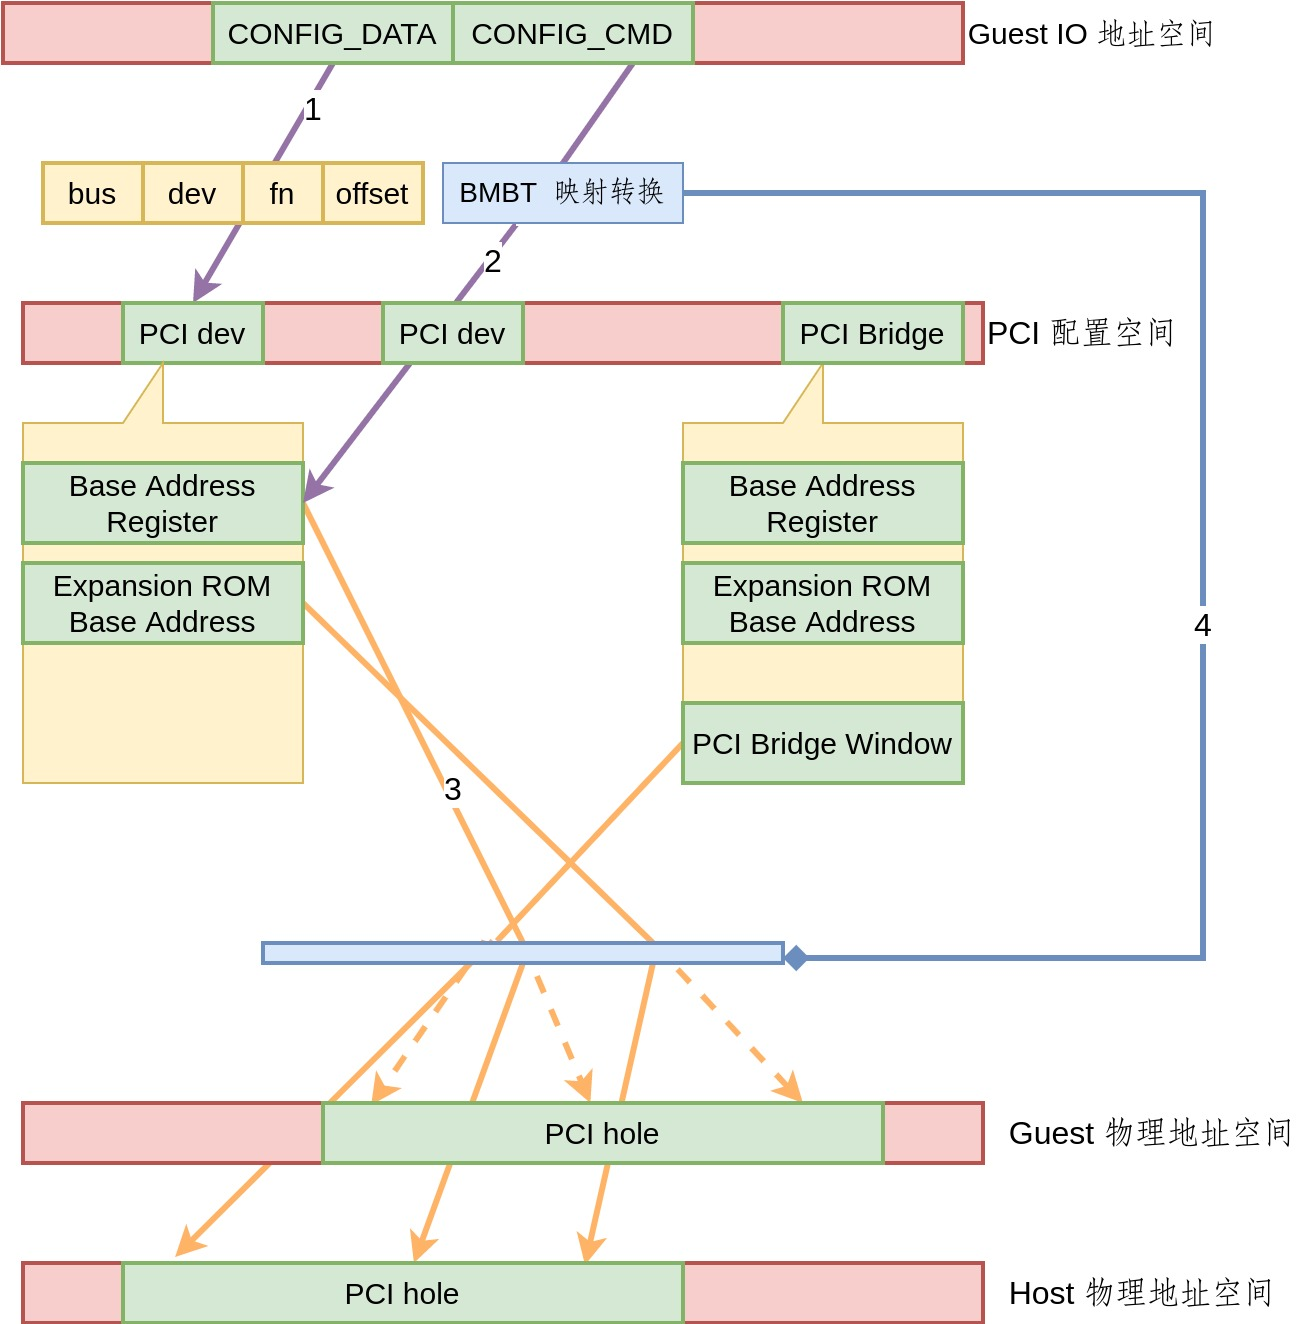
\includegraphics[width=0.5\linewidth]{../paper/images/PCIe.jpg}
		\caption{PCIe 设备直通}
	\end{figure}
	LoongArch 和 x86 对于配置空间和 mmio 空间的范围有不同的规定,因此需要进行偏移修正。
\end{frame}

\begin{frame}{设备虚拟化: 设备直通中的 DMA}
	\begin{figure}
		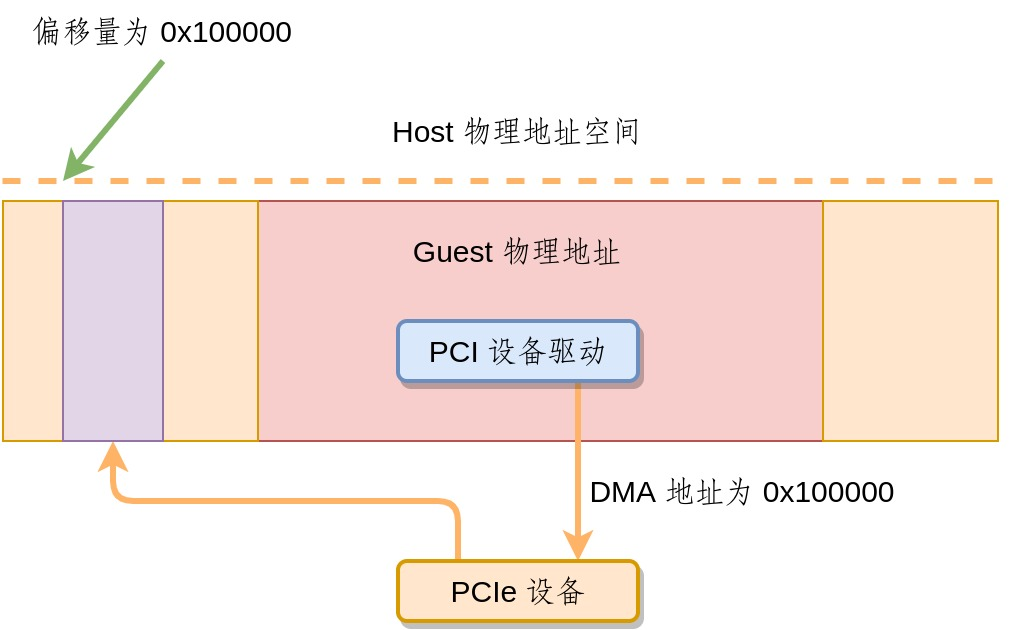
\includegraphics[width=0.48\linewidth]{../paper/images/bmbt-without-iommu.jpg}
		\hfill
		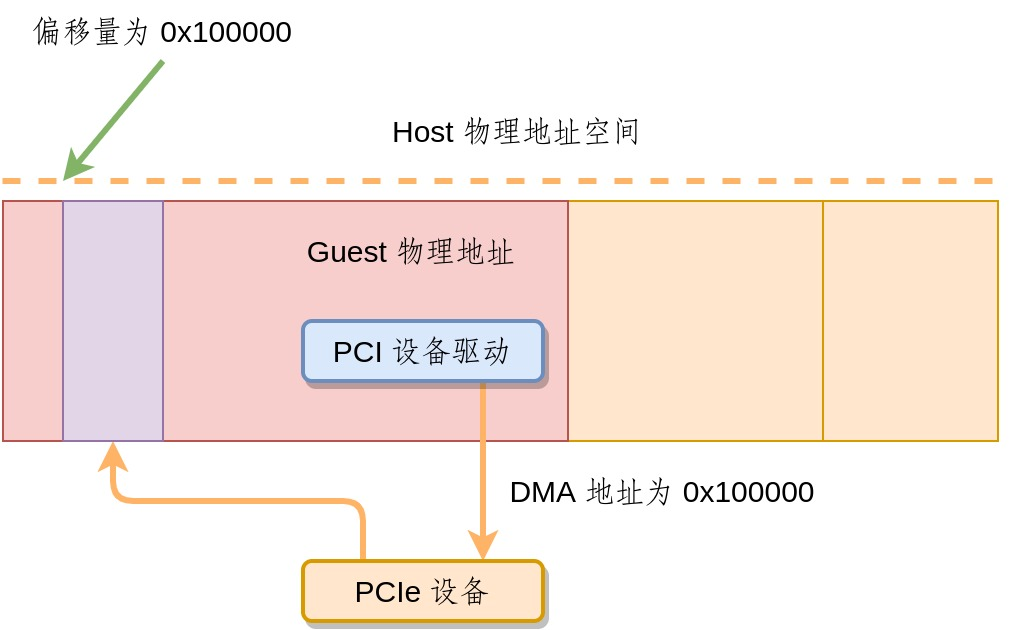
\includegraphics[width=0.48\linewidth]{../paper/images/bmbt-without-iommu2.jpg}
	\end{figure}
	左图中,没有保证 Guest Physical Address (简称 GPA)和 Host Physical Address (简称 HPA)相等,导致设备将数据拷贝到错误的位置。
\end{frame}

\begin{frame}{中断虚拟化}
	\begin{figure}
		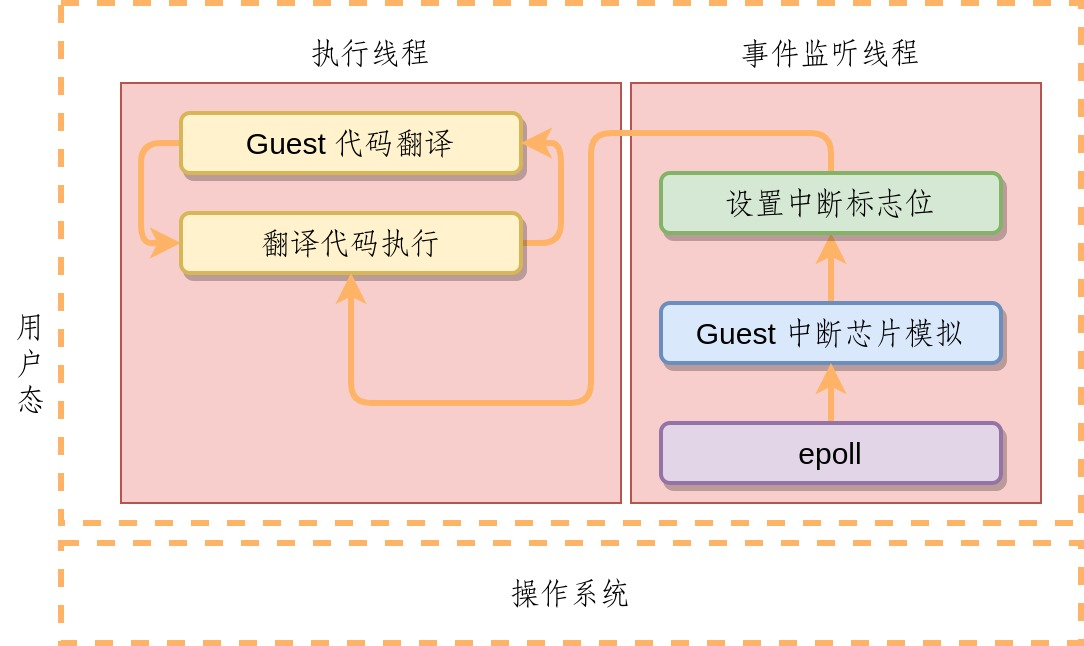
\includegraphics[width=0.5\linewidth]{../paper/images/qemu-interrupt.jpg}
		\caption{QEMU 中断软件架构}
		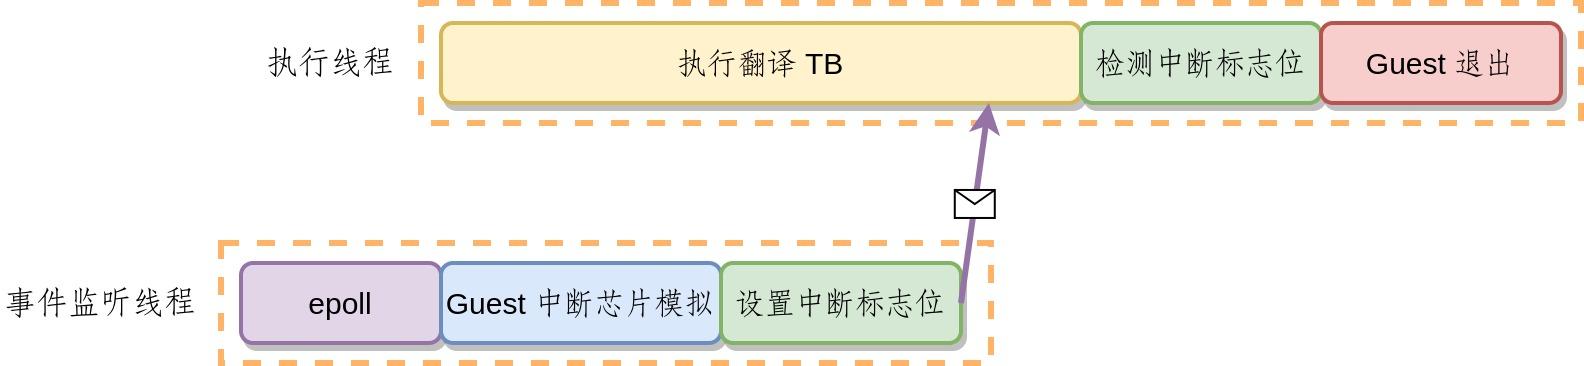
\includegraphics[width=1.0\linewidth]{../paper/images/qemu-interrupt-codeflow.jpg}
		\caption{QEMU 中断执行流程}
	\end{figure}
\end{frame}

\begin{frame}{中断虚拟化}
	\begin{figure}
		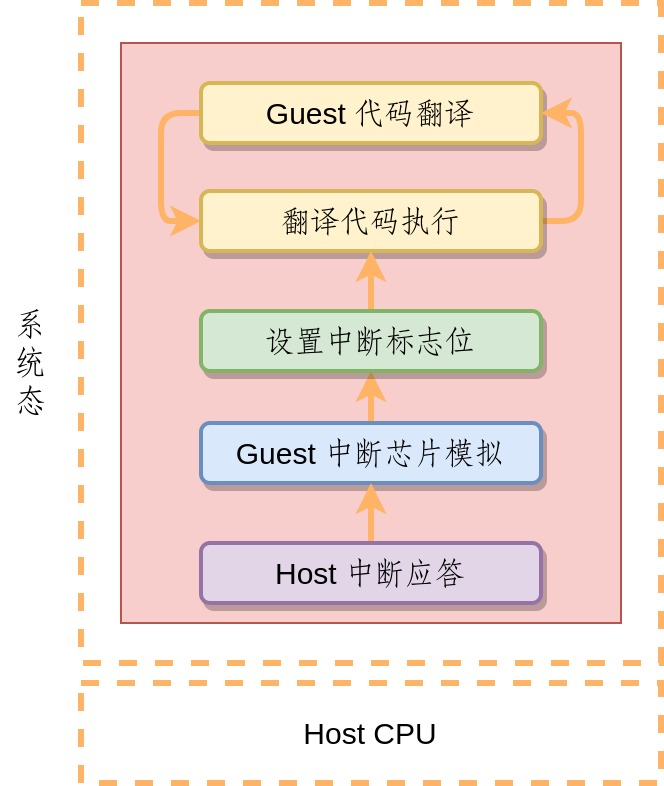
\includegraphics[width=0.35\linewidth]{../paper/images/bmbt-interrupt.jpg}
		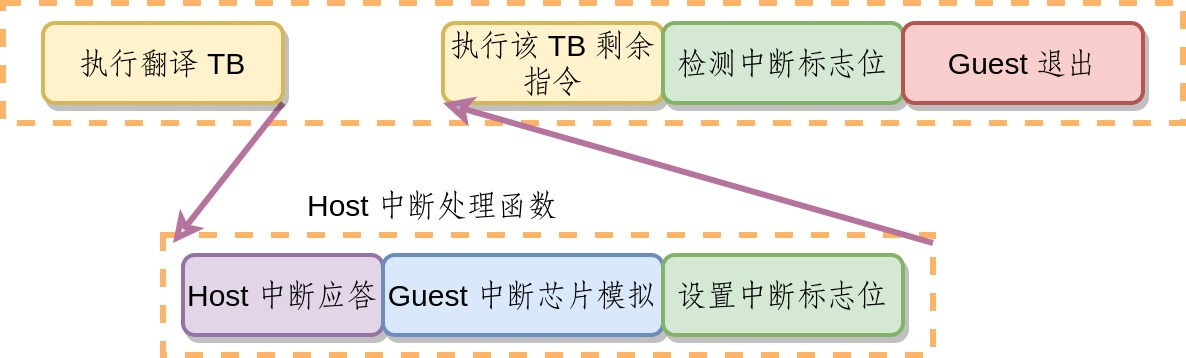
\includegraphics[width=0.6\linewidth]{../paper/images/bmbt-interrupt-codeflow.jpg}
	\end{figure}
	在裸金属上, CPU 接收中断后可以直接注入,无需额外的线程来进行事件监听。
\end{frame}

\begin{frame}{中断虚拟化}
	\begin{figure}
		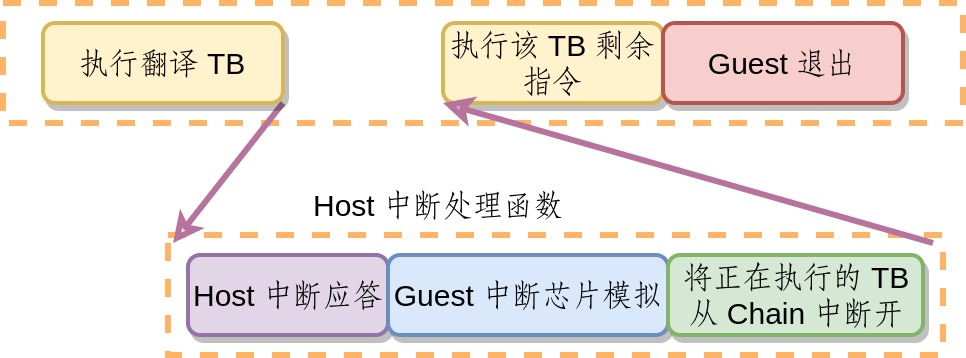
\includegraphics[width=0.7\linewidth]{../paper/images/bmbt-interrupt-codeflow2.jpg}
		\caption{消除中断标志位检测的执行流程}
	\end{figure}
	在中断处理函数中将正在执行的 TB 从 TB Chain 中断开,可以消除额外的中断标志位检测指令。
\end{frame}

\begin{frame}{内存虚拟化: TLB miss 的消除}
	\begin{figure}
		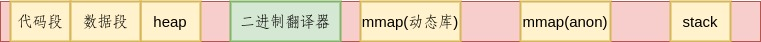
\includegraphics[width=\linewidth]{../paper/images/user-as2.jpg}
		\caption{进程级二进制翻译地址空间}
		将二进制翻译器和 Guest 的数据放到一个地址空间中, 此时 GVA 等于 Host Virtual Address (简称 HVA),Guest 的访存进行的装换为: HVA -> HPA 。
	\end{figure}
\end{frame}

\begin{frame}{内存虚拟化: TLB miss 的消除}
	\begin{figure}
		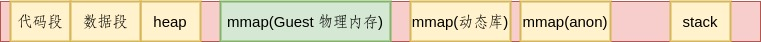
\includegraphics[width=0.8\linewidth]{../paper/images/sys-as2.jpg}
		\caption{运行在 Linux 上的系统级二进制翻译器的地址空间}
		通过 mmap 映射出来一块 Host 虚拟地址空间给 Guest 当物理内存使用。
	\end{figure}
\end{frame}

\begin{frame}{内存虚拟化: TLB miss 的消除}
	\begin{figure}
		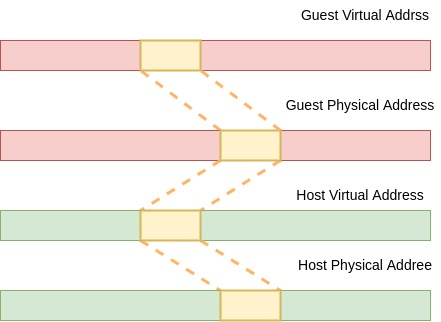
\includegraphics[width=0.45\linewidth]{../paper/images/sys-as.jpg}
		\caption{QEMU 中 Guest 的地址翻译过程}
		\begin{flushleft}
			一条 Guest 访存指令需要进行的地址装换为: GVA -> GPA -> HVA -> HPA 。
		\end{flushleft}
	\end{figure}
\end{frame}

\begin{frame}{内存虚拟化: TLB miss 的消除}
	\begin{figure}
		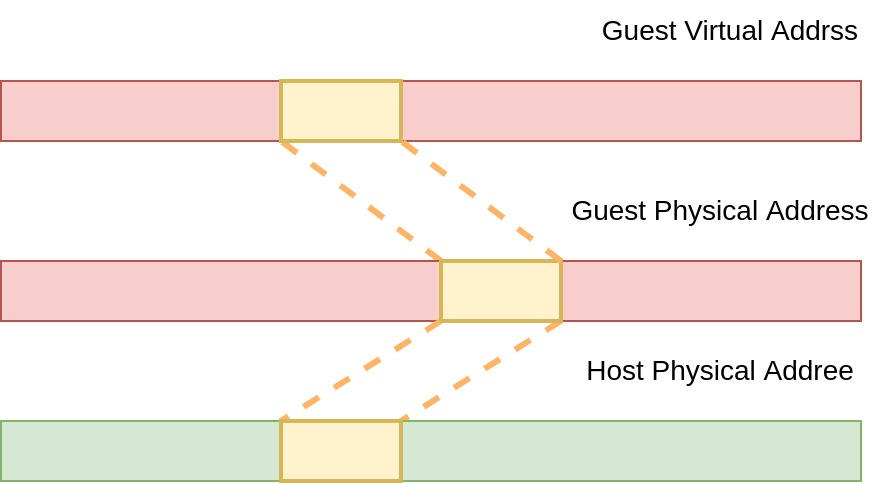
\includegraphics[width=0.6\linewidth]{../paper/images/sys-as3.jpg}
		\caption{BMBT 中 Guest 的地址翻译过程}
	\end{figure}
	BMBT 直接运行在裸金属的环境中,可以消除掉从 HVA 到 HPA 的转换
	\footnote{LoongArch 支持直接映射窗口, x86 可以关闭页表映射}
	,也就是说可以消除所有的 TLB miss 。
\end{frame}

\begin{frame}{内存虚拟化: 物理内存分配器}
	\begin{figure}
		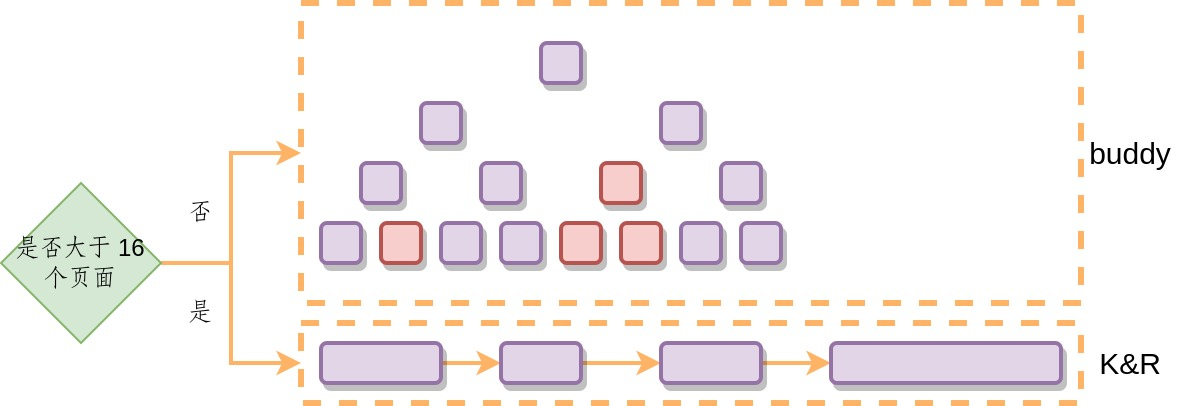
\includegraphics[width=0.8\linewidth]{../paper/images/KR-buddy.jpg}
		\caption{混合物理内存分配器}
	\end{figure}

	现代操作系统为了满足各种用户程序的需求,其物理内存分配器被设计的非常复杂。在 BMBT 中
	物理内存分配的模式单一,因此 BMBT 混合 K\&R malloc 算法和伙伴算法,在防止碎片化的前提下
	保证了分配效率。
\end{frame}

\begin{frame}{内存虚拟化: 硬件 TLB 加速}
	\begin{figure}
		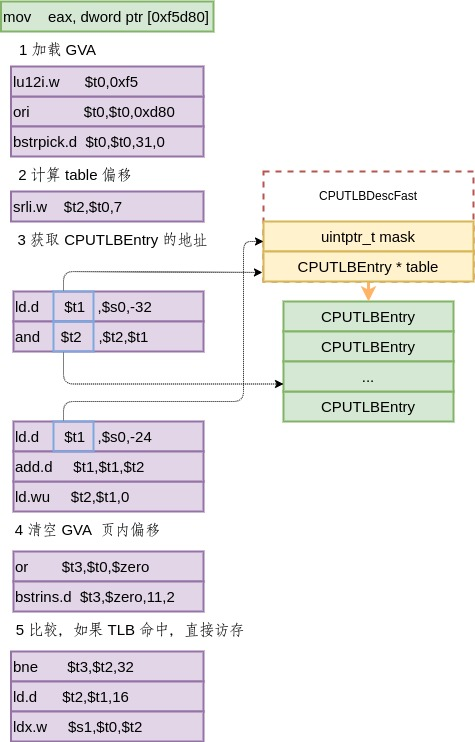
\includegraphics[width=0.35\linewidth]{../paper/images/softmmu.jpg}
		\caption{QEMU 中访存指令的翻译过程}
	\end{figure}
	一条 x86 访存指令需要 14 条 LoongArch 指令模拟。
\end{frame}

\begin{frame}{内存虚拟化: 硬件 TLB 加速}
	\begin{figure}
		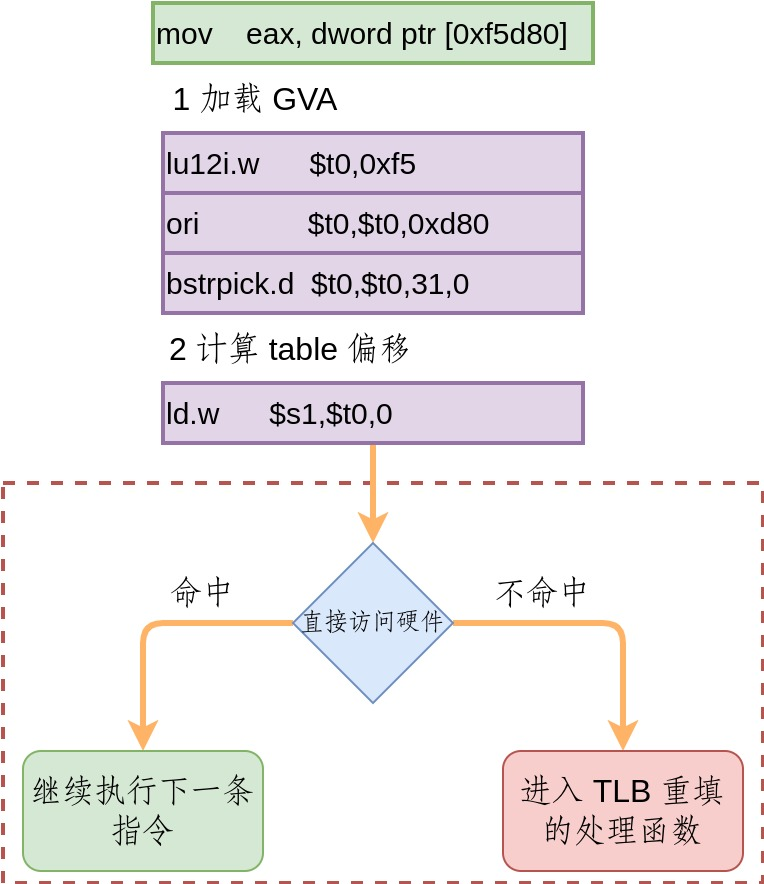
\includegraphics[width=0.4\linewidth]{../paper/images/hamt.jpg}
		\caption{硬件 TLB 加速访存后的翻译过程}
	\end{figure}
	一条 x86 访存指令被翻译为 4 条 LoongArch 指令。
\end{frame}

\begin{frame}{内存虚拟化: 硬件 TLB 加速}
	\begin{flushleft}
		访问硬件 TLB 有三种方法:
	\end{flushleft}
	\begin{enumerate}
		\item 在虚拟机中执行,例如 Captive 。
		\item 在 Dune \footcite{belay2012dune} 中执行。
		\item 直接在裸机中执行。
	\end{enumerate}
	前两种方法都引入了硬件辅助虚拟化的开销。
\end{frame}

\begin{frame}{BMBT : 裸金属二进制翻译器}
	\begin{columns}[T,onlytextwidth]
		\metroset{block=fill}
		\column{1.0\textwidth}
		\begin{exampleblock}{CPU}
			\begin{itemize}
				\item 使用 LATX 作为指令翻译引擎
			\end{itemize}
		\end{exampleblock}

		\begin{exampleblock}{设备}
			\begin{itemize}
				\item 大多数设备可以直通,无需模拟
			\end{itemize}
		\end{exampleblock}

		\begin{exampleblock}{中断}
			\begin{itemize}
				\item 无需另一个线程事件监听,直接注入中断
				\item 可以消除掉每一个 TB 中额外的中断标志位检测指令
			\end{itemize}
		\end{exampleblock}

		\begin{exampleblock}{访存}
			\begin{itemize}
				\item 消除了所有的 TLB miss
				\item 可以直接访问硬件 TLB 来加速 Guest 访存
			\end{itemize}
		\end{exampleblock}
	\end{columns}
\end{frame}

\section{性能测试}

\begin{frame}{BMBT 性能测试}
	\begin{columns}[T,onlytextwidth]
		\metroset{block=fill}
		\column{1.0\textwidth}
		\begin{exampleblock}{CPU}
			\begin{itemize}
				\item SPEC 2000 定点提升 21\% ,浮点提升 35.31\%
			\end{itemize}
		\end{exampleblock}

		\begin{exampleblock}{IO 性能}
			\begin{itemize}
				\item dd 拷贝测试中,bs 等于 1G 和 4k 的情况下分别快 83\% 和 22\%
				\item fio 写操作快 189.23\%
				\item ping 延迟显著降低
			\end{itemize}
		\end{exampleblock}

		\begin{exampleblock}{访存}
			\begin{itemize}
				\item memcpy 快 28.67\%
			\end{itemize}
		\end{exampleblock}
	\end{columns}
\end{frame}

\section{展望}

\begin{frame}{进一步的优化}
	\begin{columns}[T,onlytextwidth]
		\metroset{block=fill}
		\column{1.0\textwidth}
		\begin{exampleblock}{CPU}
			\begin{itemize}
				\item \textbf{支持多核}
			\end{itemize}
		\end{exampleblock}

		\begin{exampleblock}{设备}
			\begin{itemize}
				\item 压缩设备访问的代码路径
			\end{itemize}
		\end{exampleblock}

		\begin{exampleblock}{中断}
			\begin{itemize}
				\item 消除额外的中断检测指令
			\end{itemize}
		\end{exampleblock}

		\begin{exampleblock}{访存}
			\begin{itemize}
				\item 集成硬件 TLB 加速 Guest 访存
			\end{itemize}
		\end{exampleblock}
	\end{columns}
\end{frame}

\begin{frame}{现有工作的完善}
	\begin{itemize}
		\item 集成性能分析工具。
		\item 支持 amd64 。
		\item 支持 Windows 操作系统。
		\item 支持 ACPI 。
		\item 支持 UEFI 固件。
		\item 支持 IOMMU 。
	\end{itemize}
\end{frame}

\end{document}
